\section{Visual Components for Data Analysis}

The AnyLogic simulation software provides a number of components for analysis of the simulation model. The list includes pie charts, bar charts, different plots and diagrams.

\begin{figure}[H]
  \centering
  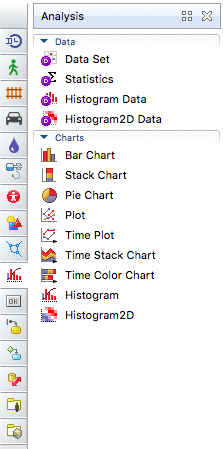
\includegraphics[height=0.5\textwidth]{img/screens/charts/charts1}
  \caption{The Analysis components for simulation model}
\end{figure}

We are going to add a time stack chart in order to see the dynamics of different populations in the model. As it can be seen from the figure, we added Susceptible, Resistant and Uncolonized values to the time stack chart. The system automatically deduces that the names refer to the values of corresponding stocks, which were created earlier.

\begin{figure}[H]
  \centering
  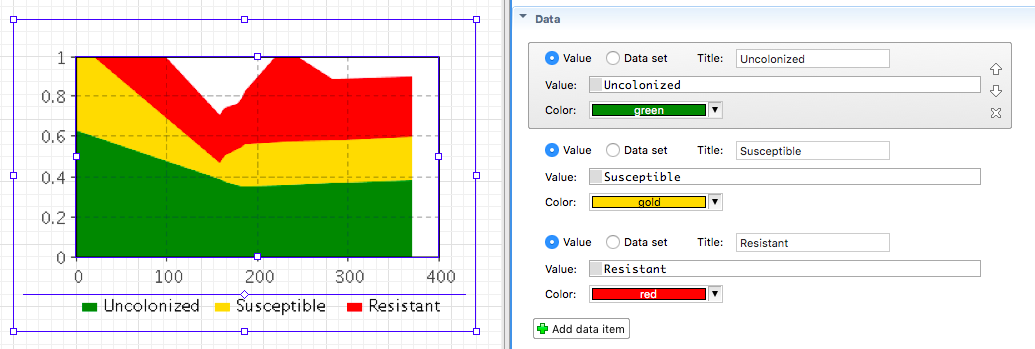
\includegraphics[width=0.8\textwidth]{img/screens/charts/charts5}
  \caption{The Analysis components for simulation model}
\end{figure}
